\documentclass[tikz,border=10pt]{standalone}
\usepackage{tikz}
\usetikzlibrary{shapes,arrows,positioning,calc,patterns,shadows,arrows.meta}

\definecolor{soscolor}{RGB}{251,188,5}
\definecolor{eoscolor}{RGB}{52,168,83}
\definecolor{maskred}{RGB}{234,67,53}
\definecolor{tokencolor}{RGB}{142,36,245}

\begin{document}
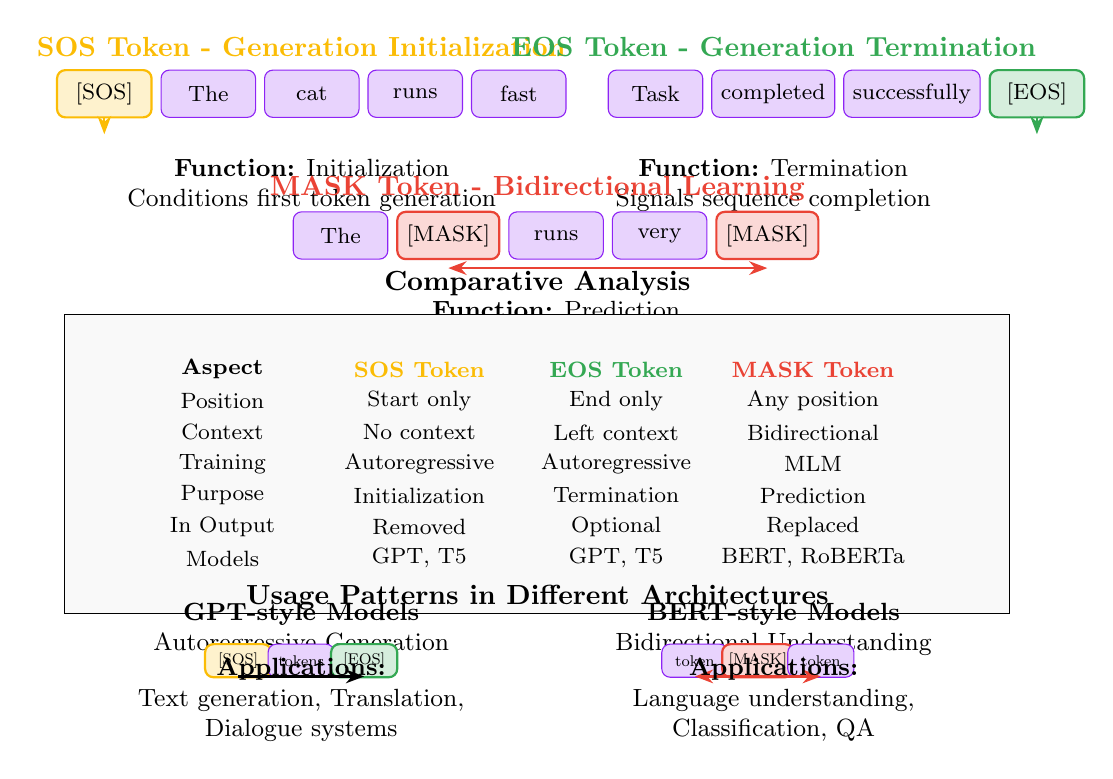
\begin{tikzpicture}[
    token/.style={rectangle, rounded corners=3pt, minimum width=1.2cm, minimum height=0.6cm, font=\footnotesize},
    sostoken/.style={token, fill=soscolor!20, draw=soscolor, thick},
    eostoken/.style={token, fill=eoscolor!20, draw=eoscolor, thick},
    masktoken/.style={token, fill=maskred!20, draw=maskred, thick},
    normaltoken/.style={token, fill=tokencolor!20, draw=tokencolor},
    label/.style={font=\small},
    title/.style={font=\large\bfseries},
    subtitle/.style={font=\normalsize\bfseries}
]

% === SPACING AND ALIGNMENT DOCUMENTATION ===
% Title: y=9.5, centered
% Token examples: SOS at y=8.2, EOS at y=8.2, MASK at y=6.4
% Function descriptions: y=7.5 for SOS/EOS, y=5.8 for MASK
% Comparison table: y=3.5, rows spaced 0.4cm apart
% Usage patterns: y=1.4 for headers, y=1.0 for examples

% Title

% SOS Token Section
\node[subtitle, soscolor] (sos-title) at (3, 8.8) {SOS Token - Generation Initialization};

% SOS example - using relative positioning
\node[sostoken] (sos-token) at (0.5, 8.2) {[SOS]};
\node[normaltoken, right=0.1cm of sos-token] (sos1) {The};
\node[normaltoken, right=0.1cm of sos1] (sos2) {cat};
\node[normaltoken, right=0.1cm of sos2] (sos3) {runs};
\node[normaltoken, right=0.1cm of sos3] (sos4) {fast};

\draw[-{Stealth}, thick, soscolor] (sos-token.south) -- ++(0,-0.2);
\node[label, align=center, below=0.4cm of sos2] {\textbf{Function:} Initialization\\Conditions first token generation};

% EOS Token Section
\node[subtitle, eoscolor] (eos-title) at (9, 8.8) {EOS Token - Generation Termination};

% EOS example - using relative positioning
\node[normaltoken] (eos1) at (7.5, 8.2) {Task};
\node[normaltoken, right=0.1cm of eos1] (eos2) {completed};
\node[normaltoken, right=0.1cm of eos2] (eos3) {successfully};
\node[eostoken, right=0.1cm of eos3] (eos-token) {[EOS]};

\draw[-{Stealth}, thick, eoscolor] (eos-token.south) -- ++(0,-0.2);
\node[label, align=center, below=0.4cm of eos2] {\textbf{Function:} Termination\\Signals sequence completion};

% MASK Token Section
\node[subtitle, maskred] (mask-title) at (6, 7) {MASK Token - Bidirectional Learning};

% MASK example - using relative positioning
\node[normaltoken] (mask1) at (3.5, 6.4) {The};
\node[masktoken, right=0.1cm of mask1] (mask-token1) {[MASK]};
\node[normaltoken, right=0.1cm of mask-token1] (mask2) {runs};
\node[normaltoken, right=0.1cm of mask2] (mask3) {very};
\node[masktoken, right=0.1cm of mask3] (mask-token2) {[MASK]};

\draw[{Stealth}-{Stealth}, thick, maskred] ($(mask-token1.south)+(0,-0.1)$) -- ($(mask-token2.south)+(0,-0.1)$);
\node[label, align=center, below=0.4cm of mask2] {\textbf{Function:} Prediction\\Uses bidirectional context};

% Comparison Table - properly aligned
\node[rectangle, draw=black, fill=gray!5, minimum width=12cm, minimum height=3.8cm] (table) at (6, 3.5) {};
\node[subtitle, above=0.1cm of table.north] {Comparative Analysis};

% Table headers - consistently spaced
\begin{scope}[every node/.style={label, font=\footnotesize\bfseries, anchor=center}]
    \node at (2, 4.7) {Aspect};
    \node[soscolor] at (4.5, 4.7) {SOS Token};
    \node[eoscolor] at (7, 4.7) {EOS Token};
    \node[maskred] at (9.5, 4.7) {MASK Token};
\end{scope}

% Table rows - properly aligned with consistent spacing
\begin{scope}[every node/.style={label, font=\footnotesize, anchor=center}]
    % Row 1: Position
    \node at (2, 4.3) {Position};
    \node at (4.5, 4.3) {Start only};
    \node at (7, 4.3) {End only};
    \node at (9.5, 4.3) {Any position};
    
    % Row 2: Context
    \node at (2, 3.9) {Context};
    \node at (4.5, 3.9) {No context};
    \node at (7, 3.9) {Left context};
    \node at (9.5, 3.9) {Bidirectional};
    
    % Row 3: Training
    \node at (2, 3.5) {Training};
    \node at (4.5, 3.5) {Autoregressive};
    \node at (7, 3.5) {Autoregressive};
    \node at (9.5, 3.5) {MLM};
    
    % Row 4: Purpose
    \node at (2, 3.1) {Purpose};
    \node at (4.5, 3.1) {Initialization};
    \node at (7, 3.1) {Termination};
    \node at (9.5, 3.1) {Prediction};
    
    % Row 5: Output
    \node at (2, 2.7) {In Output};
    \node at (4.5, 2.7) {Removed};
    \node at (7, 2.7) {Optional};
    \node at (9.5, 2.7) {Replaced};
    
    % Row 6: Models
    \node at (2, 2.3) {Models};
    \node at (4.5, 2.3) {GPT, T5};
    \node at (7, 2.3) {GPT, T5};
    \node at (9.5, 2.3) {BERT, RoBERTa};
\end{scope}

% Usage patterns
\node[subtitle] at (6, 1.8) {Usage Patterns in Different Architectures};

% GPT-style (autoregressive)
\node[label, align=center] at (3, 1.4) {\textbf{GPT-style Models}\\Autoregressive Generation};
\node[sostoken, scale=0.7] at (2.2, 1.0) {[SOS]};
\node[normaltoken, scale=0.7] at (3, 1.0) {tokens};
\node[eostoken, scale=0.7] at (3.8, 1.0) {[EOS]};
\draw[-{Stealth}, thick] (2.2, 0.8) -- (3.8, 0.8);

% BERT-style (bidirectional)
\node[label, align=center] at (9, 1.4) {\textbf{BERT-style Models}\\Bidirectional Understanding};
\node[normaltoken, scale=0.7] at (8, 1.0) {token};
\node[masktoken, scale=0.7] at (8.8, 1.0) {[MASK]};
\node[normaltoken, scale=0.7] at (9.6, 1.0) {token};
\draw[{Stealth}-{Stealth}, thick, maskred] (8, 0.8) -- (9.6, 0.8);

% Applications
\node[label, align=center] at (3, 0.5) {\textbf{Applications:}\\Text generation, Translation,\\Dialogue systems};

\node[label, align=center] at (9, 0.5) {\textbf{Applications:}\\Language understanding,\\Classification, QA};

\end{tikzpicture}
\end{document}